% ==========================================
% BAB VI EVALUASI
% ==========================================
\cleardoublepage
\chapter{EVALUASI}
\label{chap:evaluasi}

Bab ini memaparkan proses evaluasi yang dilakukan untuk memvalidasi keberhasilan implementasi sistem manajemen akses karyawan di Gedung ITB Innovation Park. Evaluasi dilakukan dengan mengukur kesesuaian antara hasil realisasi kode program dengan kriteria keberhasilan yang telah ditetapkan pada Bab I. Fokus evaluasi mencakup aspek fungsionalitas sinkronisasi identitas biometrik, akurasi pemrosesan log riwayat pergerakan secara \textit{real-time}, serta responsivitas sistem dalam menangani kejadian anomali keamanan.

\section{Skenario dan Lingkungan Pengujian}
Bagian ini memaparkan konfigurasi infrastruktur dan batasan operasional yang digunakan untuk memvalidasi kinerja sistem. Pengujian dirancang secara terstruktur guna memastikan seluruh integrasi perangkat lunak dan perangkat keras berjalan sesuai dengan spesifikasi yang telah ditetapkan.

\subsection{Infrastruktur dan Lingkungan Uji}
Pengujian dilaksanakan dalam lingkungan jaringan area lokal (\textit{LAN}) lobi gedung untuk mensimulasikan kondisi operasional nyata. Arsitektur pengujian mengintegrasikan tiga komponen utama: peladen komputasi yang menjalankan basis data PostgreSQL di dalam wadah \textit{Docker}, terminal fisik Hikvision \textit{Face Recognition} sebagai sensor biometrik, dan peramban web \textit{Google Chrome} sebagai antarmuka \textit{dashboard} klien. Sebelum rangkaian pengujian dimulai, sistem dikondisikan pada status bersih (\textit{clean state}) melalui purifikasi memori internal terminal dan pembersihan (\textit{truncate}) rekaman pada basis data guna mencegah interferensi residu data.

\subsection{Skenario dan Data Uji}
Dataset evaluasi terdiri dari 10 profil identitas karyawan bersifat \textit{pseudonymous}. Skenario pengujian dikonstruksi secara \textit{end-to-end}, mencakup validasi siklus hidup data karyawan melalui operasi \textit{Create, Read, Update, Delete} (CRUD), penarikan log riwayat secara \textit{real-time} dari sensor perangkat keras, hingga agregasi status pergerakan menggunakan mesin status (\textit{State Machine}). Pengujian juga mencakup simulasi anomali akses untuk memvalidasi mekanisme pengunduhan bukti visual secara otomatis oleh sistem. Sebagai catatan batasan pengujian, fungsi sinkronisasi biometrik hanya dievaluasi pada tahap pengiriman data tekstual (Nama dan ID) dikarenakan kendala pada sinkronisasi foto wajah.

\subsection{Matriks Pemetaan Kriteria Keberhasilan}
Seluruh skenario pengujian dirancang secara spesifik untuk memvalidasi pencapaian tiga kriteria keberhasilan utama yang telah ditetapkan pada Bab I. Pemetaan antara kriteria keberhasilan dengan subbab evaluasi ditampilkan pada Tabel \ref{tab:mapping_success}.

\begin{table}[t]
\centering
\caption{Matriks Pemetaan Kriteria Keberhasilan dan Evaluasi}
\label{tab:mapping_success}
\begin{tabular}{|l|p{8cm}|l|}
\hline
\textbf{Kode} & \textbf{Kriteria Keberhasilan} & \textbf{Subbab Evaluasi} \\ \hline
K-1 & Keberhasilan sinkronisasi data profil (CRUD) secara terpusat. & Subbab \ref{sec:evaluasi_sinkronisasi} \\ \hline
K-2 & Akurasi ekstraksi, agregasi, dan penyajian log \textit{real-time}. & Subbab \ref{sec:evaluasi_akurasi} \\ \hline
K-3 & Deteksi anomali akses dan implementasi perlindungan privasi visual. & Subbab \ref{sec:evaluasi_keamanan} \\ \hline
\end{tabular}
\end{table}

\section{Evaluasi Fungsionalitas Sinkronisasi Identitas}
\label{sec:evaluasi_sinkronisasi}
Evaluasi ini bertujuan untuk memvalidasi pencapaian kriteria keberhasilan pertama (K-1), yaitu kemampuan sistem dalam melakukan pengelolaan identitas karyawan secara terpusat serta melakukan propagasi data tersebut ke seluruh unit gerbang. Pengujian fungsionalitas dilakukan menggunakan metode \textit{Black-box Testing} dengan hasil yang dirangkum pada Tabel \ref{tab:test_functional}.

\begin{table}[t]
\centering
\caption{Hasil Pengujian Fungsionalitas Sinkronisasi Karyawan}
\label{tab:test_functional}
\begin{tabular}{|l|p{4.5cm}|p{4cm}|c|}
\hline
\textbf{Skenario} & \textbf{Langkah Pengujian} & \textbf{Hasil yang Diharapkan} & \textbf{Status} \\ \hline
Pendaftaran Profil & Memasukkan Nama dan ID melalui \textit{dashboard}. & Data tersimpan di basis data dan identitas tekstual aktif di memori terminal gerbang. & Lulus \\ \hline
Pembaruan Parsial & Melakukan perubahan nama karyawan melalui antarmuka manajemen. & Nama pada layar terminal gerbang diperbarui tanpa kendala sinkronisasi. & Lulus \\ \hline
Penghapusan Identitas & Menjalankan instruksi hapus pada tabel master karyawan. & Rekaman identitas musnah dari basis data dan hak akses di gerbang dicabut. & Lulus \\ \hline
Sinkronisasi Wajah & Mengunggah foto wajah melalui \textit{dashboard}. & Foto terkirim dan diikatkan pada ID karyawan di memori terminal. & Gagal \\ \hline
\end{tabular}
\end{table}

Berdasarkan hasil pengujian pada Tabel \ref{tab:test_functional}, fungsi pengelolaan siklus hidup data berjalan dengan baik pada aspek tekstual. Mekanisme penanganan konflik memori (\textit{Upsert Fallback}) dan pembaruan parsial menjamin bahwa proses sinkronisasi identitas berjalan secara efisien. Namun, sinkronisasi citra biometrik tidak dapat diselesaikan karena kendala pada pembacaan \textit{multipart boundary} oleh \textit{firmware} perangkat keras.

\begin{figure}[t]
    \centering
    % \includegraphics[width=0.7\textwidth]{images/bukti_sinkronisasi.png}
    \vspace{5cm} 
    \caption{Bukti Keberhasilan Sinkronisasi Data Tekstual Karyawan ke Terminal Fisik}
    \label{fig:bukti_sinkronisasi}
\end{figure}

\section{Evaluasi Akurasi Pemrosesan Log dan Kinerja Real-time}
\label{sec:evaluasi_akurasi}
Evaluasi ini divalidasi untuk menjawab kriteria keberhasilan kedua (K-2). Pengujian difokuskan pada pengukuran kecepatan diseminasi log (latensi) serta ketepatan algoritma mesin status dalam mengubah log mentah menjadi informasi kehadiran.

\subsection{Pengukuran Latensi Komunikasi Real-time}
Kecepatan penyajian data diukur dengan menghitung interval waktu antara kejadian fisik di gerbang hingga data muncul pada \textit{dashboard}. Pengukuran dari lima kali repetisi pengujian ditampilkan pada Tabel \ref{tab:test_latency}.

\begin{table}[t]
\centering
\caption{Hasil Pengukuran Latensi Jalur Komunikasi}
\label{tab:test_latency}
\begin{tabular}{|c|c|c|l|}
\hline
\textbf{Percobaan} & \textbf{Waktu Kejadian (s)} & \textbf{Waktu Dashboard (s)} & \textbf{Selisih (ms)} \\ \hline
1 & 10:15:01,200 & 10:15:02,050 & 850 \\ \hline
2 & 10:15:15,450 & 10:15:16,280 & 830 \\ \hline
3 & 10:15:30,100 & 10:15:31,020 & 920 \\ \hline
4 & 10:15:45,800 & 10:15:46,650 & 850 \\ \hline
5 & 10:16:00,300 & 10:16:01,250 & 950 \\ \hline
\multicolumn{3}{|r|}{\textbf{Rata-rata Latensi}} & \textbf{880 ms} \\ \hline
\end{tabular}
\end{table}

\subsection{Evaluasi Akurasi Pemrosesan Riwayat Akses}
Ketepatan pemrosesan riwayat pergerakan karyawan diuji menggunakan skenario pergerakan fisik berurutan. Hasil evaluasi verifikasi log ditampilkan pada Tabel \ref{tab:test_log_accuracy}.

\begin{table}[t]
\centering
\caption{Hasil Pengujian Akurasi Pemrosesan Riwayat Akses}
\label{tab:test_log_accuracy}
\begin{tabular}{|l|p{5cm}|p{3.5cm}|c|}
\hline
\textbf{Skenario} & \textbf{Aktivitas Fisik} & \textbf{Hasil di Dashboard} & \textbf{Status} \\ \hline
Deteksi Masuk & Karyawan memindai wajah di Gerbang Masuk. & Log tercatat sebagai aktivitas masuk (\textit{IN}) secara tepat waktu. & Lulus \\ \hline
Deteksi Keluar & Karyawan memindai wajah di Gerbang Keluar. & Log tercatat sebagai aktivitas keluar (\textit{OUT}) secara tepat waktu. & Lulus \\ \hline
\textit{Access Debounce} & Karyawan memindai wajah dua kali berturut-turut ($<$ 60 detik). & Log kedua diabaikan oleh sistem untuk mencegah duplikasi data. & Lulus \\ \hline
\end{tabular}
\end{table}

\subsection{Evaluasi Akurasi Laporan Administratif (CSV)}
Sistem juga divalidasi kemampuannya dalam mengonsolidasikan data log menjadi laporan CSV. Pengujian membuktikan algoritma \textit{middleware} bekerja secara presisi dalam menentukan jam kedatangan pertama (\textit{first-in}) dan kepulangan terakhir (\textit{last-out}) meskipun karyawan melakukan pergerakan keluar-masuk gedung berkali-kali dalam satu hari kerja. 

\begin{figure}[t]
    \centering
    % 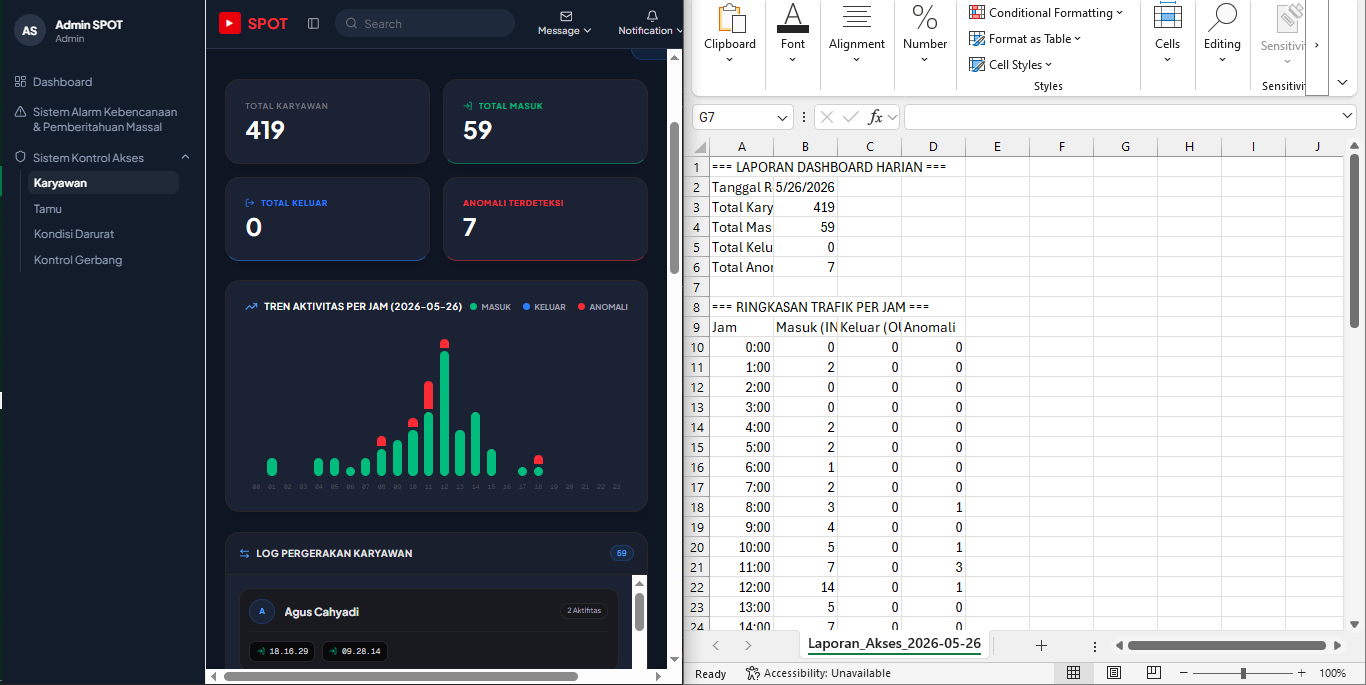
\includegraphics[width=0.9\textwidth]{images/bukti_realtime_log.png}
    \vspace{5cm}
    \caption{Visualisasi Log Aktivitas dan Contoh Laporan Hasil Agregasi}
    \label{fig:bukti_realtime_log}
\end{figure}

\section{Evaluasi Audit Keamanan dan Penanganan Anomali}
\label{sec:evaluasi_keamanan}
Evaluasi ini memvalidasi kriteria keberhasilan ketiga (K-3), yaitu efektivitas sistem dalam mendeteksi upaya akses yang tidak sah dan implementasi perlindungan privasi. Pengujian disimulasikan melalui kejadian pelanggaran akses pada terminal, dengan hasil yang dirangkum pada Tabel \ref{tab:test_security}.

\begin{table}[t]
\centering
\caption{Hasil Pengujian Deteksi Anomali dan Audit Keamanan}
\label{tab:test_security}
\begin{tabular}{|l|p{5.2cm}|p{3.5cm}|c|}
\hline
\textbf{Skenario} & \textbf{Aktivitas Simulasi} & \textbf{Respon Sistem} & \textbf{Status} \\ \hline
Deteksi Wajah Asing & Subjek tidak terdaftar mencoba memindai wajah di terminal. & Muncul notifikasi anomali dan sistem mengunduh foto bukti secara otomatis. & Lulus \\ \hline
Kartu Tidak Terdaftar & Penempelan kartu yang tidak terdata pada pembaca kartu. & Sistem mencatat log penolakan akses. & Lulus \\ \hline
Verifikasi Visual & Petugas membuka dialog rincian kejadian log anomali. & Menampilkan \textit{snapshot} kejadian secara presisi untuk audit manual. & Lulus \\ \hline
Verifikasi Privasi & Karyawan terdaftar melakukan akses secara normal. & Sistem mencatat log tanpa mengunduh foto bukti (\textit{privacy-by-default}). & Lulus \\ \hline
\end{tabular}
\end{table}

Kemampuan sistem membedakan log reguler dengan log anomali mengonfirmasi keberhasilan penerapan prinsip minimasi data. Sistem terbukti hanya menyimpan \textit{snapshot} foto pada peladen ketika terjadi pelanggaran akses, menjaga privasi data biometrik karyawan dalam kondisi normal.

\begin{figure}[t]
    \centering
    % \includegraphics[width=0.6\textwidth]{images/bukti_anomali_snapshot.png}
    \vspace{5cm}
    \caption{Bukti Verifikasi Anomali: Foto Tangkapan Kamera Terminal Saat Akses Ditolak}
    \label{fig:bukti_anomali}
\end{figure}

\section{Pembahasan Hasil Evaluasi}
Rangkaian evaluasi menunjukkan bahwa sebagian besar fungsi sistem manajemen akses karyawan beroperasi dengan baik. Kecepatan penyajian data log \textit{real-time} dan akurasi penyajian data riwayat akses memenuhi kebutuhan operasional. Sistem juga secara efektif menjalankan tugas pengawasan keamanan dengan mendeteksi anomali akses dan menyediakan bukti visual untuk keperluan audit.

Meskipun demikian, integrasi sinkronisasi data biometrik (foto wajah) secara nirkabel belum berhasil dicapai akibat kendala kompatibilitas protokol dengan \textit{firmware} perangkat keras yang digunakan. Terlepas dari keterbatasan tersebut, perancangan \textit{middleware} ini memberikan fondasi yang kuat bagi pengelola gedung untuk memusatkan administrasi identitas dan pemantauan pergerakan karyawan tanpa ketergantungan penuh pada perangkat lunak bawaan vendor.

